\chapter{意义的湍流：有限计算中的多尺度表征与结构重整}
\label{chp:meaning_turbulence}

有限智能面对的困难并不是把一个无限世界逐项装进有限存储，而是在有限时间、容量和访问带宽内，持续保留对当前任务有用的差异、关系与因果前提。旧稿借“卷曲”“湍流”和“重整化”描写这种压力，本章把这些比喻重建为可以检查的计算对象：任务相关压缩、层级编码、跨尺度耦合、结构编辑以及外部记忆。我们先规定状态、查询、预算和误差，再讨论粗粒化如何保留可回答性，快状态与慢结构如何双向更新，何种拥塞会引发级联失稳。物理语言只用于帮助辨认多尺度现象，不充当证明。HSF--HD在这里给出一般状态动力学模型族；AgentOS的$h(t)$、$E$、$\Theta$、$\Psi$、SPC、TCE、CCM、Boundary、Offloading与外部记忆$M_e$只是其中一种可审计实现，而不是所有智能系统必须采用的器官表。

\section{有限表示：任务距离、压缩与可实现性}
\label{sec:geometry_limit}

我们把时刻$t$的内部状态写成$z_t=(h_t,E_t,\Theta_t,A_t,M_t)$。其中$h_t\in\mathbb{R}^{d_h}$是连续活动表示，$E_t$是带类型边与身份键的有限关系集，$\Theta_t$是参数或规则状态，$A_t$是当前可调用接口集合，$M_t$是受容量约束的内部记忆。环境历史记为$x_{0:t}$，任务规格记为$q_t\in\mathcal Q$；二者都可能随时间改变。这个定义没有要求一切智能都采用向量加图，只要求具体模型声明其状态空间、可观测量和允许的更新。一个表示是否“靠近”另一个表示，不能由图形相似或欧氏距离单独决定，而应由任务查询的可区分性决定。给定查询族$\mathcal Q_t$、答案损失$\ell_q$和读出器$r_q$，我们定义任务距离
\begin{equation}
 d_{\mathcal Q_t}(z,z')=\sup_{q\in\mathcal Q_t}\left|\ell_q(r_q(z),y_q)-\ell_q(r_q(z'),y_q)\right| .
\end{equation}
它是无量纲的性能差异；若损失带单位，则须先按任务容差归一化。两个状态在某一查询族上距离很小，只说明它们对这些查询近似等价，不能推出内部结构同构，更不能推出对未来所有问题都等价。

有限实现通过编码器$c_t:x_{0:t}\mapsto z_t$完成。若状态最多占用$B_m$字节、单步更新至多消耗$B_c$次基本操作、响应延迟不超过$B_\tau$秒，我们把$B=(B_m,B_c,B_\tau)$称为实现预算。压缩不是把“无限语义”神秘地折进有限体积，而是在预算内选择一个等价类代表。其任务失真定义为
\begin{equation}
 D_t(c,r)=\mathbb E_{q\sim\mu_t}\!\left[\ell_q(r_q(c(x_{0:t})),y_q)\right],
\end{equation}
其中$\mu_t$是当期查询分布。若$\mu_t$、答案标准或接口改变，$D_t$也改变；因此旧表示的有效性必须重新评估。所谓“捷径”是对常见查询减少访问步数的索引、缓存或结构边，而不是物理虫洞。它节省的是算法路径长度和响应时间，是否降低焦耳能耗还取决于硬件、数据搬移与缓存命中，不能从路径变短直接推出。

有限性至少产生三种不同压力。容量压力来自可写状态接近$B_m$；访问压力来自相关信息虽存在却不能在$B_\tau$内取回；结构压力来自旧索引不再匹配新的查询分布。三者的症状都可能表现为答非所问，但处置不同：容量不足需要压缩或卸载，访问拥塞需要索引与调度，结构失配需要重编码或重建绑定。以跨年法律问答为例，删除失效条文也许释放容量，却不能修复版本键缺失；增加向量库也许扩大存储，却不能保证检索到适用法域。模型必须保留文书日期、辖区、效力层级和引用链，读出时再按查询身份绑定，而不能把语义相似当成规范有效。

我们据此区分局部结构网络与全局分布表示。局部网络$E_t$显式保存身份、角色和约束，适合追踪“谁在何时依据什么”；分布状态$h_t$整合大量弱证据，适合相似性检索和不完全观测下的连续估计。二者不是互斥本体，也不能从脑区分工类比推出机制等同。它们通过任务相关身份键、绑定算子$b_t$、耦合算子$K_t$和读出接口$r_q$联合：结构为分布读出限定合法对象，分布证据为结构候选提供评分。若身份键冲突，系统应拒绝或保留多假设，而不是用高相似度覆盖明确关系。

工程上我们用对照实验确认“卷曲”是否真的形成有效捷径。先记录基线的查询准确率、尾延迟、读取字节数和更新成本，再逐个移除缓存边、层级摘要或外部记忆接口。如果移除后只增加内部步数而任务结果不变，它是效率结构；如果准确率下降，它承载了任务信息；如果训练集改善而分布外查询恶化，它可能只是过拟合。由此，抽象被限定为在声明查询族和预算下的有损压缩，而不是“抽象必然等于几何折叠”的形而上断言。我们能够检验的是任务保持、资源变化和失效边界，而不是由一个成功预测反推整个内部世界的唯一形状。

\section{容量边界：遗忘、干扰与运行资格}
\label{sec:axiom_of_compactness_and_pathology}

有限系统必须遗忘，但遗忘并不等同于损坏。设记忆项$i$占用$b_i$字节，预计查询概率为$p_i(t)$，回答价值为$v_i(t)$，取回代价为$c_i(t)$，保存决策$a_i\in\{0,1\}$。一个简单的选择问题是，在$\sum_i a_i b_i\le B_m$下最大化$\sum_i a_i[p_i v_i-\lambda c_i]$。这是工程模型而非智能公理；它揭示保存策略依赖未来查询分布和价值估计。若$p_i$估错，系统会删掉低频但关键的安全规则；若$v_i$只取短期奖励，系统会牺牲长期承诺。因而记忆治理还需不可删除集合、版本保留期和审计策略，不能把容量优化交给单一相关度分数。

我们把运行病理分为覆盖、不可达和漂移。覆盖是写入新内容后旧内容被参数或缓存更新破坏，可用旧任务回放检测；不可达是内容仍在但索引、权限或接口不能找到，可用已知键的取回测试定位；漂移是同一标识的解释随上下文或版本改变，可用跨期一致性和来源链检测。三类问题都可能被笼统称为灾难性遗忘，但它们作用在不同对象上。覆盖需要隔离或稳定化更新，不可达需要修复寻址，漂移需要版本化语义。仅扩大上下文窗口往往只缓解瞬时不可达，还可能增加注意力竞争和错误绑定。

旧稿把无外部检索的语言模型描述成“无痛感、无目的”的平坦系统，并把幻觉归因于不能卷曲。这种推论混合了经验主张与本体判断。我们只讨论可观测机制：冻结参数的生成器仍可在激活状态中形成暂时结构，也可借缓存、工具和控制器获得跨步状态；但若没有可靠来源绑定、未知检测和提交门，它会在证据不足时继续生成。幻觉率受训练分布、解码规则、检索质量、校准方法和任务评价共同影响，不能由是否具有体验直接推导。是否存在痛感属于另一个研究层级，不作为本章工程结论。

对AgentOS实例，$h(t)$承载当前分布状态，$E$承载显式关系，$\Theta$承载慢参数，外部记忆$M_e$保存可版本化记录。SPC可提出候选，TCE可按目标和约束选择，CCM可监控冲突，Boundary控制跨域读写，Offloading决定何时把内容移入$M_e$。这些名字有助于把故障分账：例如检索缺失属于$M_e$与接口，未经授权写入属于Boundary，目标漂移属于TCE或上游规格。换一种系统完全可以用其他组件完成同样功能，所以不能把组件缺失等同于智能缺失。

运行资格由一组门槛而非单个“紧致性”判定。我们至少要求：状态更新在资源预算内完成；高风险结论能给出来源或明确拒答；结构版本与读出版本相容；外部动作经过授权；在监测到输入分布、任务目标或接口变化时触发降级。设负载$u_t$、尾延迟$L_{.99,t}$、错误率$e_t$和证据覆盖率$g_t$，资格谓词可以写作
\begin{equation}
 \mathrm{Ready}_t=[u_t\le u_{\max}]\wedge[L_{.99,t}\le L_{\max}]\wedge[e_t\le e_{\max}]\wedge[g_t\ge g_{\min}],
\end{equation}
其中阈值由任务风险给出，不是跨任务常数。谓词失败时应停止、降级或请求外部确认，而不是继续生成以维持表面流畅。

容量边界应通过负载曲线验证。我们逐渐增加并发、历史长度、关系密度和版本数量，分别记录吞吐、尾延迟、遗漏、错绑与拒答。在到达物理内存上限之前，系统可能先因索引扇出、锁争用或注意力稀释失效；这正说明“有限体积导致热熔断”不是充分诊断。反例也必须保留：一个容量小但任务窄、索引稳定的系统可以长期可靠；一个容量巨大但来源混乱的系统仍会高频错答。有限性要求选择与治理，却不预先决定某一种几何、硬件或心理属性。

\section{层级表征：粗粒化、查询保持与结构摘要}
\label{sec:geometric_mold_renormalization}

多尺度表征从可检查的编码链开始。设第$k$层状态空间为$\mathcal Z_k$，编码器$R_k:\mathcal Z_k\to\mathcal Z_{k+1}$把细粒度状态压成摘要，解码或细化接口$D_k:\mathcal Z_{k+1}\times C_k\to\widehat{\mathcal Z}_k$在上下文$C_k$下恢复任务所需细节。$R_k$不必可逆；我们要求的是查询保持：对指定查询集$\mathcal Q_k$，
\begin{equation}
 \epsilon_k=\sup_{q\in\mathcal Q_k}\left|\ell_q(r_q(z_k),y_q)-\ell_q(r_q(D_k(R_kz_k,C_k)),y_q)\right|\le\bar\epsilon_k.
\end{equation}
误差阈值$\bar\epsilon_k$由任务容差给出。若查询集改变，原摘要可能失效；因此摘要必须附带生成版本、适用查询和来源范围，而不能被当成脱离任务的“意义结晶”。

粗粒化可以是聚合、采样、低秩投影、图商、程序归纳或统计充分量。它们的成立条件不同。低秩投影要求相关变化集中在保留子空间；图商要求被合并节点对目标查询近似不可区分；充分统计量依赖声明的概率族；程序摘要则依赖执行语义。我们不把它们统一叫作物理重整化并由名称取得正确性。只有当层间变换、误差界和验证数据被明确给出时，重整化群的语言才提供有用类比：多次变换后保留哪些量、哪些扰动被抑制、哪些误差被放大。

以急诊分诊为例，底层记录包括症状出现时间、生命体征、药物、过敏史和测量来源。上层摘要可以输出风险级别与关键证据，但不能把“胸痛”与“既往心梗”仅因语义接近合并为同一节点。身份、时间和否定词应保留在局部结构网络$E$中；大量弱信号可由分布表示$h$整合；绑定接口把风险读出连接到具体患者和具体测量。若上层请求追溯，$D_k$不是凭空复原被删信息，而是通过来源指针访问原记录。没有来源时，系统只能报告摘要，不得生成伪造细节。

结构摘要还必须处理变化。令结构$E_k(t)$、度量$G_k(t)$、查询分布$\mu_k(t)$随时间变化，层间误差的总导数不能只写状态项，而应包含
\begin{equation}
 \frac{d\epsilon_k}{dt}=\partial_z\epsilon_k\,\dot z_k+\partial_E\epsilon_k\,\dot E_k+\partial_G\epsilon_k\,\dot G_k+\partial_\mu\epsilon_k\,\dot\mu_k+\partial_t\epsilon_k.
\end{equation}
这里的导数在结构固定区间内成立；节点增删、模式迁移和权限变更是离散事件，需在事件边界重新定义空间并复核误差。忽略这些项，会把目标变化造成的失效误判为模型噪声，也会把旧指标上的稳定误判为任务稳定。

层级并非天然树形。一个事实可以同时属于时间线、因果链、组织权限和主题聚类；强迫它只有一个父节点会丢失交叉关系。我们采用带类型的多层图：层内边保存局部结构，层间边标记聚合、实例化、证据或控制关系，全局分布表示提供柔性相似度。查询计划先用结构边限定合法候选，再用分布读出排序，必要时回到细粒度证据。这样既避免把所有内容平铺扫描，也避免把摘要当作唯一真相。所谓“高阶结构被包进空腔”在实现上对应的是可追溯引用和受控省略，不是信息无损消失。

验证层级表征需要三类基线。第一类是无压缩基线，用于测量节省和失真；第二类是同容量平面索引，用于确认收益确来自层级而非参数增加；第三类是随机或错误层级，用于排除训练泄漏。指标至少包含查询正确率、校准误差、追溯成功率、更新传播延迟与资源成本。还要构造反例：低频安全规则、跨层身份冲突、摘要过期和多父关系。若系统只在平均查询上更快，却在这些关键情形丢失约束，就不能称为有效抽象。层级表征的结论因此是条件性的：它在声明查询、预算和更新协议内减少计算，而不是为所有语义规定唯一尺度。

\section{双向更新：证据聚合、目标约束与结构修订}
\label{sec:dynamical_loop_ricci_sculpting}

多尺度系统同时包含快状态与慢结构。令$z_k(t)\in\mathbb R^{d_k}$是第$k$层连续状态，$A_k(t)$是带类型的结构算子，$u_k(t)$是外部输入，$g_k(t)$是任务目标，$G_k(t)$是度量或预条件器。结构固定时，我们采用
\begin{equation}
 \dot z_k=F_k(z_k,A_k,u_k,g_k,t)+U_k(z_{k-1})+D_k(z_{k+1}),
\end{equation}
其中$U_k$汇聚下层证据，$D_k$施加上层约束。这个方程是模型假设，不是由物理定律推出；各项必须映射到同一状态空间并保持量纲或归一化尺度一致。上行项不自动代表“真实”，下行项也不自动代表“意志”，它们都可能携带误差。

慢结构依据累计证据更新。设候选编辑集合为$\Delta\mathcal E_k$，编辑$\delta$的任务收益估计为$\widehat B_t(\delta)$，迁移成本为$C_t(\delta)$，风险为$R_t(\delta)$，则可在审计窗口内选择
\begin{equation}
 \delta_t^*=\arg\max_{\delta\in\Delta\mathcal E_k}\bigl[\widehat B_t(\delta)-\lambda C_t(\delta)-\rho R_t(\delta)\bigr].
\end{equation}
节点、边或模式改变后，状态维度与合法操作也可能改变，所以结构更新是离散事务，不应伪装成处处可微的“逆里奇流”。实际过程应在影子结构上重放历史任务，通过后再原子切换；失败时保留旧版本和回滚路径。目标下降只证明在测试目标上的改进，不等于现实任务成功。

下行约束的作用是缩小合法集合、分配注意或触发额外观测。例如“不能向未授权对象泄露病历”应通过Boundary约束检索与输出，而不是只在生成末尾降低某些词的概率。上行创新则可提出旧结构没有的候选关系，例如多个故障工单共同指向一项依赖。候选先作为假设进入$E$的待证区，只有得到来源、时间与反事实检查后才转为承诺边。由此，证据聚合与目标控制互相作用但不相互替代：目标不能制造事实，证据也不能自行决定价值优先级。

离散实现以步长$\Delta t$更新快状态：$z_{n+1}=z_n+\Delta t\,F(z_n,A_n,u_n,g_n,t_n)$。若$F$在有效域内对$z$的Lipschitz常数为$L$，显式更新至少需要选取与$L$和稳定域相容的步长，并监测越界；结构切换时则重新初始化或投影状态。异步系统还要记录输入时间、目标版本和结构版本，避免把后来规则错误地施加到早先事件。没有这些条件，连续模型的局部稳定不能自动传递给部署中的队列、重试和并发写入。

我们用新闻核验说明闭环。底层收集多个来源的原句、发布时间和编辑记录；中层绑定同一事件的参与者和地点；上层目标要求在速度、准确与伤害风险间取舍。若新来源与旧摘要冲突，上行项提高多假设权重，下行约束要求延迟高风险发布，结构事务把“已确认”边降级为“争议”。系统不是把流形熨平，而是显式改变状态、关系和承诺级别。随后通过新证据校准：若持续误报同类来源，才考虑修改来源可靠度结构；一次冲突不足以重写全部规则。

双向闭环的验证采用消融和扰动。移除上行通道，系统会僵化于旧结构；移除下行通道，候选会越过权限和任务边界；取消版本控制，异步更新会产生不可复现结果；禁止回滚，结构试验的风险会外溢。我们分别测量检测延迟、误绑定、约束违反、结构切换收益和回滚成功率。只有这些指标共同改善，才能说双向更新有效。把一切变化解释成“宏观意志雕刻几何”会遮蔽具体责任，也无法告诉工程系统在何处拒绝、重试或恢复。

此外，结构候选应设最小观察窗，防止一次偶然误差触发永久编辑；紧急安全规则可以例外，但须记录触发者、作用域和到期条件，并在事后回放中复核。

\section{多尺度流动：非线性、拥塞与语义级联}
\label{sec:meaning_cascade}

“意义湍流”在本章指一种计算现象：输入、记忆和结构更新跨尺度耦合后，小扰动可能通过重试、竞争和错误摘要被放大，导致任务状态频繁切换。为避免把流体术语当作证明，我们定义无量纲负载指数
\begin{equation}
 \chi_t=\frac{\lambda_t\tau_m\kappa_t}{C_{\mathrm{eff},t}},
\end{equation}
其中$\lambda_t$是单位时间有效事件数，$\tau_m$是事件保持或处理时间，$\kappa_t$是平均耦合扇出，$C_{\mathrm{eff},t}$是同一时间窗内可服务的有效容量。各量按一致时间单位测量，故$\chi_t$无量纲。它不是流体雷诺数，也不保证存在统一临界值；它只是比较到达、滞留、传播和容量的运行指标。

当$\chi_t$较低且结构版本稳定，事件通常在局部完成，更新路径可预测。随着负载上升，队列等待使上下文过期，过期结果触发重试，重试又占用容量；若关系扇出高，一个身份错绑会传播到多个摘要和缓存，形成正反馈。此时输出看似“跳跃”，原因却可能是普通的排队与版本竞争，而非深层创造。我们用因果图区分三条链：输入激增导致服务拥塞，目标频繁改变导致结构抖动，局部错误经摘要传播导致全局冲突。三者需要限流、目标冻结窗和来源回溯等不同干预。

\begin{figure}[htbp]
    \centering
    
\includegraphics[width=0.82\linewidth,height=0.54\textheight,keepaspectratio]{image/thought.png}
    \caption{多尺度思维活动的意境图；本章不把涡旋形态视为计算机制的证据}
\end{figure}

级联可以向上也可以向下。向上级联把多个局部异常合并为新的风险类别：例如不同设备的温升、振动和丢包共同支持“供电异常”假设。向下级联则由上层策略改变许多局部行为：进入安全模式后降低采样率、冻结写入并请求人工复核。两种方向都要保留作用域。若上层摘要把不相关设备合并，错误策略会大面积传播；若底层只上传平均值，稀有故障会被淹没。因此系统需要身份键、异常通道和反向追溯，而不是单纯追求更强耦合。

非线性来自门控、饱和、离散提交和共享资源，而不必诉诸神秘场。一个候选在阈值附近可能因微小证据改变从“不提交”跃迁为“提交”；多个任务争用同一外部工具会让延迟骤升；图编辑改变合法动作集合会使后续轨迹分叉。我们分别把连续置信变化、离散决策和资源等待记录下来。若只看最终文本，会把三种来源混成“灵感”或“混乱”。可审计系统应能回答：哪个阈值被越过、哪个版本生效、哪个资源饱和、哪些下游读出受到影响。

一个具体反例是突发新闻。大量内容相似的转发会使分布表示高度一致，但它们可能都来自同一未经核实的首发。若把相似度当独立证据，系统会快速形成错误宏观摘要。结构网络必须追踪来源谱系，把共同祖先折叠为一份证据；全局表示仍可帮助聚类，但不能决定证据数量。相反，两个措辞不同、来自独立现场的报告可能提供更强支持。级联控制因此依赖来源独立性、时间顺序与身份绑定，而不是信息量表面的多少。

我们通过相图而非诗意描述验证多尺度流动。实验轴包括$\lambda$、$\kappa$、缓存期限、目标切换率和有效容量；输出包括吞吐、尾延迟、错误放大率、恢复时间与任务得分。重复实验确定从局部处理到拥塞、振荡或降级的区域，并报告置信区间。若增加容量只推迟而不消除失稳，需检查反馈结构；若降低耦合减少错误却损害必要协作，需寻找选择性边界。这里的“湍流”是对复杂运行区的辅助名称，结论来自可重复的负载与扰动实验，而不是从流体外观推导智能规律。

\section{内化与外化：压缩、卸载与跨期连续}
\label{sec:bidirectional_folding_hrf}

有限智能既把外部规律内化为快速预测，也把内部状态外化为可持久记录。内化不是把世界完整复制进参数，而是使编码器、检索器或控制策略在常见条件下减少额外观测；外化也不是把“自我”简单搬到数据库，而是把可命名内容连同来源、版本和权限写入外部介质。设内部状态$I_t=(h_t,E_t,\Theta_t)$，外部记忆$M_e(t)$由记录$r_i=(k_i,v_i,s_i,\nu_i,a_i)$构成，依次表示身份键、内容、来源、版本和访问策略。二者通过写入$W_t:I_t\to M_e$与取回$R_t:M_e\times q_t\to\widehat I_t$连接；任何写回或读回都可能有损、有延迟，也可能因权限失败。

内容应放在内部还是外部，取决于更新频率、访问概率、时延、隐私和一致性，而不是一条普遍的“向内卷曲/向外展开”规律。我们为候选内容$i$定义放置代价
\begin{equation}
 J_i(a)=p_iL_i(a)+\alpha U_i(a)+\beta S_i(a)+\gamma P_i(a),\qquad a\in\{\mathrm{in},\mathrm{out},\mathrm{both}\},
\end{equation}
其中$L_i$是预计访问延迟，$U_i$是更新与同步成本，$S_i$是失效风险，$P_i$是隐私或合规风险。各项先按任务阈值归一化，权重由应用给出。高频稳定规则可内化，低频大对象可外化，高风险承诺可在内部保留索引而把签名原件外置；但网络中断、外部服务变更和密钥失效必须进入部署假设。

AgentOS实例中的Offloading决定候选迁移，Boundary检查读写权限，CCM比较内部承诺与外部版本，SPC形成取回或写入方案，TCE依据目标和风险提交。$h(t)$可暂存当前解释，$E$保存身份与依赖，$\Theta$提供稳定读出，$M_e$承担大容量、跨会话和可审计记录。这里最重要的是接口契约：取回结果必须附带来源和版本，写入必须幂等或拥有事务键，缓存必须声明期限。若把检索文本无条件拼入状态，攻击内容、旧版本和身份冲突会越过Boundary，外部记忆反而成为失稳源。

跨期连续依赖可验证的继承关系，而非存储数量。设会话$t$结束时提交承诺集合$C_t$及其哈希、来源与未决项，下一会话先读取可访问的$C_t$，再在新证据下生成$C_{t+1}$。系统应区分延续、修订、撤销与遗忘：延续需要引用原承诺，修订需要给出差异及理由，撤销需要保留审计痕迹，遗忘则明确说明信息不可得。仅凭相似文本生成一个“像过去的我”的回答，不证明状态连续；相反，一个换了模型却能可靠继承承诺和边界的系统，可能在任务意义上保持更强连续性。

组织中的外化更说明问题。事故复盘、设计决策、值班手册和代码库共同构成团队记忆，却由不同人员、工具和权限维护。分布表示有助于找到相似事件，结构网络则保存责任、版本、依赖和批准链。人员离职时，口头经验若未外化会丢失；文档存在但索引失效则不可达；手册与代码不一致则发生漂移。把所有信息塞进单个模型不能消除这些治理问题。外化质量要用检索覆盖、版本一致、责任可追溯和恢复演练衡量。

内化与外化的实验需要跨期和故障条件。我们比较纯内部、纯外部与混合系统在断网、缓存污染、权限收紧、模型升级和模式迁移时的表现，记录正确率、恢复时间、未授权暴露和承诺保持。若外部记忆只在正常网络下提高平均分，却在版本冲突时静默错答，它不构成稳健连续；若内化规则提升速度却阻碍法规更新，也需配置失效门。结论是：压缩与卸载共同扩展有限系统的有效历史，但连续性来自身份、来源、版本和读写协议，而不是从存储介质本身推导。

\section{元控制的形成：从瞬态响应到自我模型}
\label{sec:pure_geometric_dynamics_ontogeny}

元控制不是突然出现的“宏观意志奇点”，而是系统开始把自身状态、能力和约束纳入决策对象。我们区分四个可观察阶段。第一阶段只有瞬态响应，输入到达后状态改变但不跨事件保留；第二阶段形成重复可调用的模式，类似缓存或习惯；第三阶段产生跨情境摘要，能够把多个实例绑定到同一规则；第四阶段建立自我模型，系统预测某个策略对自身资源、承诺和未来可行性的影响。阶段是分析框架，不声称所有智能都按同一路径发育，也不从生物发育类比推出计算必然。

经典的铃声与食物例子可用条件预测表达。令$x_t$为铃声特征，$y_t$为食物到达，$p_\theta(y_{t+1}\mid x_t,c_t)$为上下文$c_t$下的预测。重复配对更新$\theta$后，铃声成为预测线索；若环境改变，预测误差应使关联衰减。这里形成的是条件关系，不等于系统理解实验者意图。只有当它能表示“当前关联可能失效”、主动选择检验并根据结果调整学习率时，才接近元控制。自我模型因此至少需要对自身预测误差、资源和更新可靠度的二阶估计。

我们把元状态写为$m_t=(\widehat c_t,\widehat r_t,\widehat u_t,\widehat\sigma_t)$，分别表示能力范围、剩余资源、当前承诺和不确定度。策略选择为
\begin{equation}
 a_t=\arg\min_{a\in\mathcal A_t} \mathbb E[J_{g_t}(z_{t+1})\mid z_t,m_t,a]+\lambda\,\mathrm{Risk}(a\mid m_t),
\end{equation}
合法动作集$\mathcal A_t$受Boundary和现实接口限制。若$m_t$校准良好，系统会在证据不足或资源耗尽时拒答、分解任务或卸载；若过度自信，它会越界提交；若过度保守，则可能把可做任务全部拒绝。目标函数下降只说明内部估计改善，必须再与现实反馈比较。

\begin{figure}[htbp]
    \centering
    
\includegraphics[width=0.82\linewidth,height=0.54\textheight,keepaspectratio]{figure/curl.png}
    \caption{结构重整的示意图；卷曲仅作为局部关系被重新邻接的视觉辅助}
\end{figure}

自我模型同样依赖局部结构与全局分布的联合。结构网络明确列出工具权限、数据边界、未完成承诺和行动依赖；分布状态汇聚模糊的难度、熟悉度和异常感。任务相关身份把“我能调用的数据库”与“用户提到的数据库”区分，绑定接口把能力估计关联到特定版本与环境。不能从脑部某区域的活动推断系统必有对应模块，也不能把一个中心节点称为自我。自我读出可以分布在多个组件，只要能在决策时形成一致、可追溯的约束。

元控制还需要承诺管理。内部候选、语言输出和外部动作具有不同可逆性：候选可以丢弃，输出可能被人采纳，现实动作可能不可撤销。系统应在每级设置提交门，记录谁授权、依据何在、如何补偿。一次高置信预测不能自动越过外部授权。AgentOS可由CCM检测承诺冲突、TCE选择修复策略、Boundary阻止越权动作；其他架构可以用事务协调器或策略引擎实现同一功能。

验证元控制要测试“知道不知道”，而不仅是平均任务分。我们构造能力边界内、边界附近、明显超域和工具故障四类任务，测量成功、拒答、无谓拒绝、越权尝试和不确定度校准。再改变工具版本与资源预算，检查自我模型是否随环境更新。若系统只是背诵固定能力说明，却在真实权限变化后仍宣称可用，就没有在线自我模型；若它能定位失败原因、选择替代路径并在恢复后重新验证，才显示了可操作的元控制。

自我模型还应区分“尚未尝试”“尝试失败”和“原则上不可执行”。三者需要不同的探索、修复与拒绝策略；把它们压成一个低置信度会浪费资源，也会模糊责任边界。

\section{载体协同：表示、网络与组织结构}
\label{sec:co_evolution_of_physical_substrate}

计算状态必须由某种载体实现，但实现关系不是语义结构与物理拓扑的一一同构。我们区分任务图$G_T=(V_T,E_T)$、逻辑执行图$G_L$和物理或组织图$G_P$。任务图描述身份、依赖和约束，逻辑图描述算子与消息，物理图描述处理器、存储、网络或责任主体。映射$\phi:V_T\to2^{V_P}$可以是一对多、多对一并随负载改变。只要读写语义、故障边界和时序条件被满足，同一任务结构可以部署在不同载体上；反之，相似物理网络也能承载完全不同的任务。

协同设计的目标是满足端到端约束。设逻辑边$e$的消息量为$b_e$字节、物理路径延迟为$l_e$秒、失败概率为$p_e$，节点计算时间为$c_v$秒。一个部署的期望代价可写为$J=\sum_v c_v+\sum_e(b_e/B_e+l_e)+\rho R$，其中$B_e$是带宽，$R$综合故障与合规风险。这个式子是近似工程模型；队列相关性、重试与并发会使代价非加性。优化部署不能只最小化平均延迟，还要保护尾延迟、隔离域和恢复路径。

生物脑的局部回路、长程连接和可塑性提供了“结构与活动共同变化”的经验证据，却不证明数字系统必须复制脑区，也不证明某一算法与某一脑机制等同。我们保留可迁移的问题：局部处理如何减少通信，远程连接如何选择性建立，损伤后如何重路由，慢结构如何由快活动塑造。答案必须在目标系统中重新测量。把缓存称为海马、把路由器称为丘脑，并不会增加机制解释。

在分布式AgentOS实例中，$h(t)$可在加速器上更新，$E$可在关系存储中维护，$\Theta$由模型服务承载，$M_e$由对象存储和日志系统组成；SPC、TCE、CCM与Boundary可由多个服务协作而非固定机器。关键是跨组件身份与版本：一个候选方案必须引用产生它的模型、结构快照和输入；提交后要能追踪到外部动作。若只复制向量而遗漏身份键，全局分布表示会与局部结构脱绑定，得到流畅但不可审计的结果。

组织也构成载体。客户支持、工程、法务和运营各有局部状态与权限，工单与会议形成耦合接口。组织图的“边”有带宽、等待时间和责任含义；增加群聊连接未必提高协作，可能增加中断和责任模糊。有效设计把任务相关身份、升级条件和决策权写清，并允许低风险局部自治。一个中心协调者可以改善一致性，却可能成为瓶颈和单点故障；完全去中心化可提高韧性，却需要冲突解决与共同日志。

载体协同的边界由可替换性实验检验。我们更换模型、存储、网络路径或责任小组，保持接口契约和任务集不变，观察任务质量、延迟与恢复是否仍在容差内。若更换导致大幅失效，说明隐藏耦合尚未建模；若不同载体都能满足约束，则支持功能层的多重实现，但不意味着内部状态整体同构。载体研究因此应报告映射、接口、时序和故障，不用“形质硬件化”掩盖具体部署选择。

协同还要计算观测成本。为了确认一个远端模块健康，心跳、追踪和一致性检查本身占用带宽与存储；监测太少会延迟故障发现，监测太多会挤占任务流量。系统按风险设置采样率，并让监测数据与业务身份分域保存。若组织载体参与决策，还需把交接等待、值班覆盖和人工确认纳入同一端到端时序，而不是只测机器调用。这样才能把“共同演化”落实为接口随任务与载体证据一起修订，而非假定硬件或组织自然适配语义。

\section{计算介质：存储墙、互连与异构加速}
\label{sec:silicon_medium_phase_transition}

计算介质影响可实现的状态动力学，最直接的限制往往不是算术峰值，而是数据移动。设一次操作读取$b_r$字节、写入$b_w$字节、执行$f$次运算，算术强度为$I=f/(b_r+b_w)$。当$I$低于硬件的计算带宽比时，性能受存储带宽限制；增加算力单元不会线性提速。长上下文注意、图遍历和外部检索都可能触及不同层次的存储墙，因此“更高维拓扑处理器”不是充分方案，首先要识别数据布局、复用和互连瓶颈。

三维堆叠、高带宽存储、近存计算、光互连和专用加速器各有收益与约束。堆叠缩短部分路径却增加热密度和制造复杂性；近存计算减少搬移却限制算子与精度；光互连提供带宽但转换、缓存和控制仍有成本；异构芯片提高特定算子效率却增加编译、调度和一致性负担。我们不把这些技术解释为“空间折叠”或“物理虫洞”，而用字节、秒、瓦、错误率和寿命等真实单位比较。

介质选择还改变故障模型。易失存储断电丢失，非易失介质有写入寿命与保持误差，模拟器件受漂移与噪声影响，分布式存储受网络分区影响。若状态$h$允许近似误差，而身份关系$E$必须精确，二者可能需要不同介质：向量计算可容忍低精度，授权边和事务日志不能因量化随机翻转。局部结构与全局分布表示的差异在这里转化为数据类型、容错和一致性要求，而不是脑区对应。

异构调度把逻辑算子$o_i$分配到设备$d_j$。我们需同时考虑执行时间$t_{ij}$、迁移量$m_{ij}$、实际能耗$e_{ij}$与可用精度$a_{ij}$，在任务误差和延迟约束下求解放置。焦耳能耗$e_{ij}$是实测物理量，不能与信息熵、活动强度或目标代价混称为“认知能量”。若优化目标只含内核时间，系统会频繁搬移状态，端到端反而更慢；若只含能耗，可能牺牲实时任务。部署结论必须随工作负载和设备版本重新测量。

一个典型流程包含分布编码、结构检索、候选生成、约束检查和外部调用。分布编码适合加速器批处理，结构检索受随机访问和索引影响，约束检查可能需要精确CPU逻辑，外部调用则受网络支配。把所有步骤压到单一阵列会产生资源错配。较稳健的方案以任务身份和版本元数据贯穿异构流水线，并在跨设备边界设置校验；局部结果可缓存，但结构变更后必须失效。

评价新介质不能只展示峰值。我们报告端到端吞吐、尾延迟、数据移动量、平均和峰值功耗、热降频、错误校正、生命周期写入量及软件迁移成本。还要与同工艺、同容量和同精度基线比较。若某设备只在静态小图上有效，却在结构频繁变化时重新编译过慢，应明确适用域。介质可以扩大某类动力学的预算包络，却不自动带来抽象、意志或自我；这些能力仍取决于表示、更新、接口和验证。

生命周期评价还要包含模型与数据更换。加速器若只能支持固定形状或少数算子，短期速度优势可能被重新量化、编译和数据转换抵消。系统应在需求变化、批量变化和故障降级下复测，而不是把首版基准永久外推。对于安全关键任务，还要证明低精度误差没有跨过结构提交阈值，并为精确复核保留独立路径。介质层的可观测计数器应与上层任务事件绑定，否则功耗峰值、错误校正和输出失真之间仍无法建立因果定位。

\section{HRF计算模型：编码、解码与跨尺度误差}
\label{sec:hrf_math}

我们把层级化重整流HRF定义为一组有向层状态与可训练接口，而不是独立物理场。第$k$层状态$z_k\in\mathbb R^{d_k}$，结构$E_k$属于有限图集合$\mathcal G_k$，编码器$R_k:\mathbb R^{d_k}\times\mathcal G_k\to\mathbb R^{d_{k+1}}$，解码器$D_k:\mathbb R^{d_{k+1}}\times C_k\to\mathbb R^{d_k}$。不同层维数可以不同；若状态含概率，接口还须保持归一化；若含类型关系，图变换须保存合法类型。HRF是模型族，各实例需要说明层数、状态类型和更新频率。

训练目标由任务、重建、结构和资源项组成：
\begin{equation}
 \mathcal L=\mathcal L_{\mathrm{task}}+\sum_k\alpha_k\|P_kD_k(R_k(z_k),C_k)-P_kz_k\|_{G_k}^2+\sum_k\beta_k\mathcal L_{\mathrm{struct},k}+\gamma\mathcal C_{\mathrm{resource}}.
\end{equation}
$P_k$只投影任务相关分量，$G_k\succeq0$定义无量纲加权误差，结构损失检查身份、类型和约束，资源项可以包含字节与延迟但须先归一化。重建项小不意味着任务成功；任务项下降也不证明结构忠实。不同主张由不同测试集和对照验证。

若用谱粗粒化，设层图拉普拉斯$L_k$为对称半正定，$U_{k,r}$含最小$r$个特征值对应向量，可令$R_kz=U_{k,r}^{\top}z$。这种保留低频的解释要求图近似无向、度量明确且任务信号确实平滑。对有向因果图、强异配网络或稀有异常，低频未必承载关键任务。我们必须用随机投影、任务监督池化和不压缩基线比较，不能从“低频等于宏观意义”直接得出。

\begin{figure}[htbp]
    \centering
    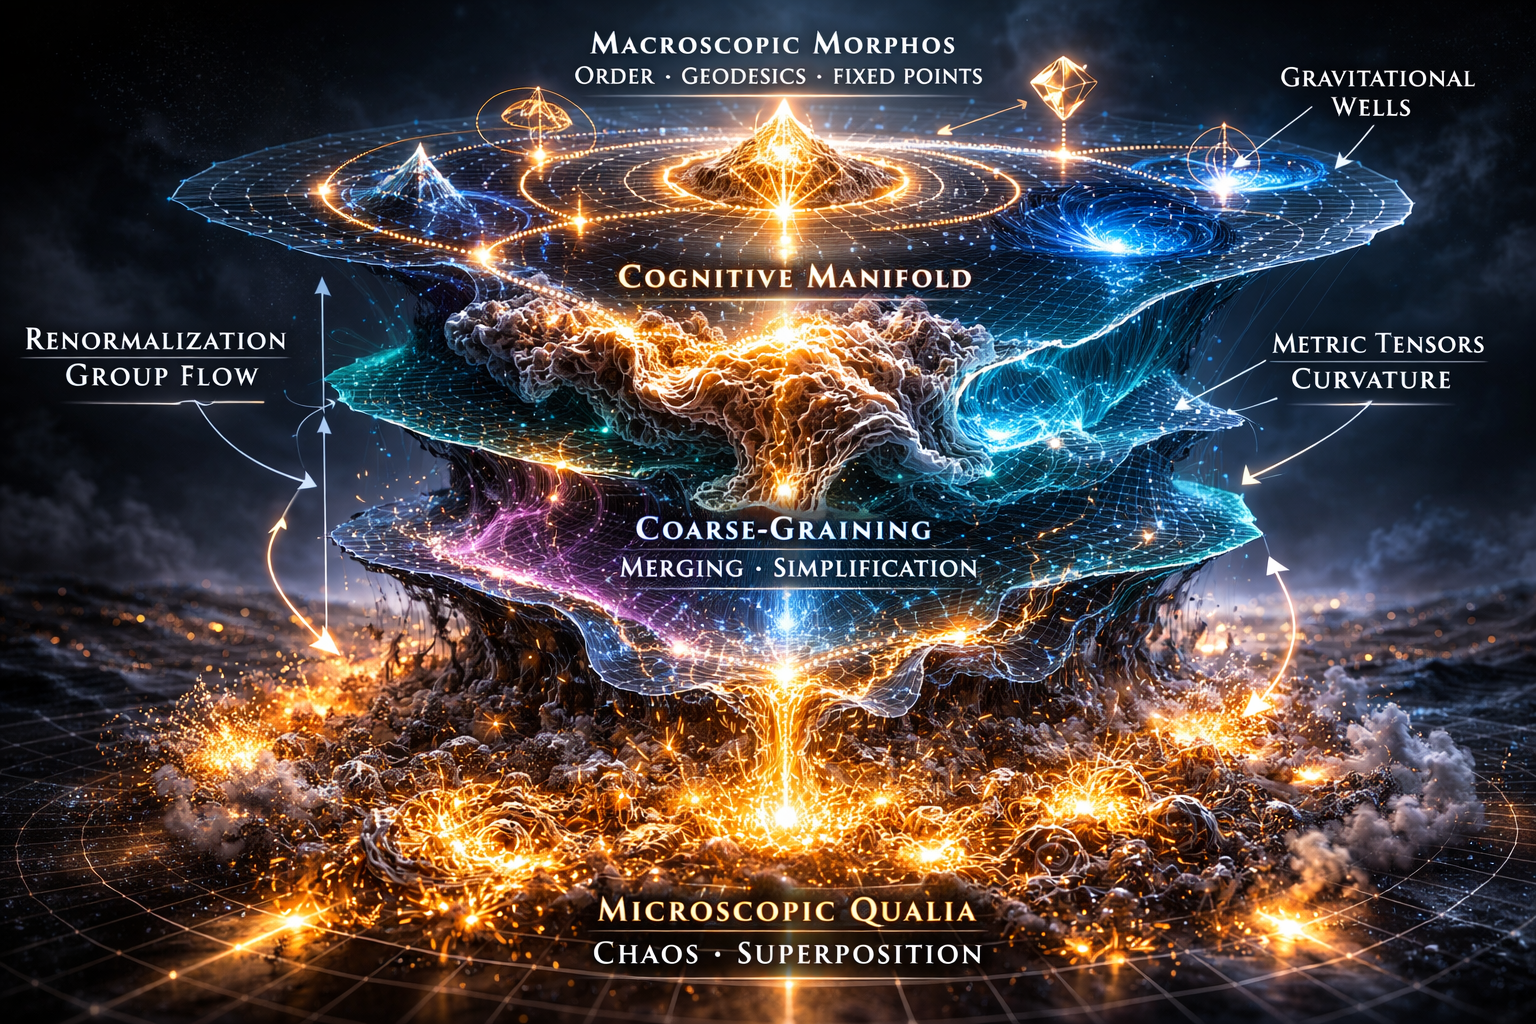
\includegraphics[width=0.82\linewidth,height=0.54\textheight,keepaspectratio]{image/hrg.png}
    \caption{HRF多层编码与反馈的示意图}
\end{figure}

多层误差可由Lipschitz条件传播。若读出$r$、解码器$D_k$在有效域内常数分别为$L_r,L_{D_k}$，第$k$层局部误差为$\epsilon_k$，则末端误差可上界为若干$\epsilon_k$乘后续常数的和。只有当乘积受控时，增加层数才不会放大误差。所谓不动点$R(z^*)=z^*$也只在同维映射、有效闭集和收缩条件下由Banach定理保证；一般跨维编码没有这个结论。即使收敛，不动点也可能是无信息常数，仍需任务和结构测试。

在线运行同时含连续或逐步状态更新与离散结构更新。固定结构下可用$z_{k,n+1}=z_{k,n}+\Delta t_kF_k(\cdot)$，步长按局部稳定与时延选择；每隔$N_k$步或在漂移触发时提出结构候选，影子验证后切换$E_k$版本。各层异步时，消息必须携带事件时间、状态版本和结构版本，过期消息按策略丢弃或重算。忽略这些语义，数学上正确的层间映射也会在部署中混合不同世界状态。

HRF验证分为可回答性、可追溯性和资源性。我们比较原始细粒状态与各级摘要对同一查询的答案差异，追踪答案能否返回证据，测量每层的字节、延迟与更新成本。再施加查询漂移、结构编辑、异常稀有事件和消息乱序，观察误差界是否仍覆盖实测结果。若界失效，系统应扩大保留维度、切换解码路径或降级到细粒度处理。HRF因此是一套可组合压缩与控制接口，不是把语义提升为物理高维的证明。

层数和瓶颈宽度通过验证选择。增加层级可能提高复用，却同时增加消息、版本和误差传播；扩大维度可能降低重建误差，却增加访问与更新成本。我们在同一预算下扫描层数、维度与更新周期，绘制任务误差、资源成本和追溯成功率的帕累托前沿。选择点由风险容差而非单一平均分决定。对高风险查询，系统可绕过摘要直接读取证据；对低风险高频查询，则允许使用缓存读出。两条路径必须共享身份与版本，避免快速路径返回旧世界、慢速路径返回新世界。

编码器和解码器也需进行方向性检验。$D_kR_k$接近恒等只检查细节往返，$R_kD_k$接近恒等则检查一个上层状态能否稳定细化后再聚合；两者通常都只在有效子集成立。若解码器具有强生成先验，它可能产生看似合理却无来源的细节，所以追溯指标必须与重建指标并列。我们对被压缩掉的变量做干预，观察上层答案是否变化，以识别摘要真正忽略了什么；若关键因果变量被平均掉，即使静态重建漂亮，也应拒绝该层级设计。

HRF还应提供运行时不确定度。每级摘要附带覆盖范围、误差估计、时间戳和失效标志；跨层组合时按依赖传播，而不是把多个置信度简单相乘。当异常超出训练域，系统提升细粒读取比例并冻结结构写入，待证据恢复后再放开。这一协议把数学误差界变成可执行的降级动作，也允许审计者定位是哪一层、哪一版本首先越界。

\section{跨层耦合：上行创新、下行约束与闭环稳定}
\label{sec:hierarchical_flow_unification}

层级系统的价值不在于层数多，而在于不同时间尺度能够交换必要信息而不相互淹没。令$z=(z_0,\ldots,z_K)$，固定结构区间内的耦合模型为
\begin{equation}
 \dot z_k=f_k(z_k,u_k,g_k,t)+B_{k,k-1}\phi_{k-1}(z_{k-1})+B_{k,k+1}\psi_{k+1}(z_{k+1}).
\end{equation}
上行映射$\phi$把局部证据、异常或新候选传给高层，下行映射$\psi$把目标、预算和合法集合传给低层。矩阵$B$声明接口维度和耦合强度。该式并非把所谓“质”与“形”统一成物理场，而是把可观察的消息路径写进状态方程；若接口是离散消息，则应使用混合系统而非强行求连续导数。

上行创新必须与证据等级绑定。局部模块可以提出“现有类型不足”“出现新关系”或“摘要无法解释残差”，但候选不能直接成为全局事实。系统记录产生候选的输入、模型、结构版本和不确定度，并在独立数据或外部观测上验证。一个传感器突变可能是新事件，也可能是漂移或故障；只有比较邻近传感器、校准记录和因果时序后，才决定建立新节点、调整参数或标记设备异常。这样保留了旧稿所说的自底向上涌现，却不把异常自动神圣化为意义。

下行约束也不是任意压制。高层目标$g_k$应被编译成可检查的局部约束，例如速率上限、权限集合、必经验证和风险预算。若约束互相冲突，低层不应静默选择，而应返回不可满足证据。以供应链计划为例，上层要求交付日期、成本上限和合规来源；局部调度在没有可行供应商时必须报告空集，而不是伪造方案。目标提供选择标准，但不能改变库存事实或取消物理运输时间。

稳定性只在明确条件下讨论。若无输入的线性化系统为$\dot{\delta z}=J\delta z$，$J$的特征值实部均为负可给出局部指数稳定；有界输入下还需输入到状态稳定或增益条件。层间时延$\tau_{ij}$、饱和、目标切换与结构编辑都会改变结论。我们不把某个标量目标下降称为“自由能最小化后必然稳定”，因为目标可以随时间变，局部下降也可能通过共享资源伤害其他层。验证需要扰动所有相关通道并测量恢复域。

异步实现尤其容易制造伪闭环。高层依据版本$v$发出约束，低层可能已切换到$v+1$；上行摘要抵达时对应的原事件已经撤销。每条消息因此携带事件时间、因果前驱、结构版本与幂等键。接收方按水位线决定等待、丢弃、补偿或重算。对不可交换的结构编辑使用串行化或冲突图；对可交换统计更新允许并行。所谓跨层“共振”若不能指出消息版本和处理顺序，就无法区分真正协同与重复反馈。

闭环失稳常见于增益过大、时延过长和目标抖动。高层看到短期误差便频繁改规则，低层尚未适应又收到新规则，观测因延迟继续恶化，形成追逐。缓解方法包括滞回、最小驻留时间、速率限制和影子评估，但它们都会牺牲响应速度。我们在阶跃、脉冲、周期和结构突变四类扰动下记录超调、恢复时间、约束违反与任务效用，并比较无耦合、单向耦合和双向耦合。只有双向系统在目标域内给出更好权衡，才支持跨层统一的工程主张。

系统还需为不可恢复情形设计降级。当证据通道断开，上层应降低承诺等级；当目标服务不可用，低层按最后已知安全策略运行；当结构版本无法对齐，暂停不可逆动作并保存事件。AgentOS可以让CCM检测跨层冲突、TCE重规划、SPC提出替代、Boundary封锁外部执行，但这些功能也可由其他控制架构实现。闭环稳定来自条件、协议和测试，不来自组件名称或物理类比。

\section{全局联合状态：分层算子、读出与可观测性}
\label{sec:holographic_unification}

全局状态不是“每个局部都含有整体”的全息复制，而是把各层状态、结构与接口放进一个联合模型。设
\begin{equation}
 Z_t=(z_{0,t},\ldots,z_{K,t},E_{0,t},\ldots,E_{K,t},V_t),
\end{equation}
其中$V_t$记录版本、权限和事件时间。联合更新$Z_{t+1}=F_t(Z_t,U_t,G_t)$由层内算子、层间耦合和离散结构事务组成，外部读出$y_t=H_q(Z_t)$随查询$q$选择相关层。这个表示是分析便利，不要求系统把$Z_t$集中存放；在分布式实现中，它可能只能通过一致快照近似获得。

“整体”首先由任务身份连接。局部结构网络保存对象、关系与因果前驱，全局分布表示保存跨来源的柔性统计，绑定算子把同一实体在各层的实例联合，耦合接口传递摘要和约束，读出接口再按问题选取视图。若身份解析错误，增加更宽的联合向量不会修复；若只有结构而无分布证据，系统难以处理噪声与相似变体。因此联合不是把两类表示混成一个无差别张量，而是保留类型后协同。

能否从输出识别内部状态涉及可观测性。在线性近似$Z_{n+1}=AZ_n+BU_n, y_n=CZ_n$中，有限时域可观测矩阵$\mathcal O=[C^\top,(CA)^\top,\ldots]^{\top}$满秩，才可从理想输出重构状态；实际系统还受噪声、离散结构和非线性影响。许多内部自由度对当前查询不可观测，这并不意味着它们不存在，也不允许从少量成功输出断言整体机制唯一。我们应报告可辨识的任务子空间及其条件。

全局一致性也不是所有副本每时每刻相同。强一致、因果一致、最终一致和会话一致适合不同操作。授权撤销和资金扣减可能要求强一致或串行事务，推荐缓存可以接受短暂陈旧，审计日志则要求不可篡改的因果顺序。把所有层锁成单一同步步长会牺牲可用性；完全放任则产生承诺冲突。系统按关系类型选择一致性，并在读出中暴露快照时间与不确定度。

下行读出存在遗漏风险。一个高层摘要可能满足常规问题，却隐藏稀有但关键的局部状态。我们为关键事件设置旁路通道：异常、权限冲突和安全约束不经平均聚合直接上报，同时仍保留去重和来源检查。反过来，高层目标也通过作用域下发，避免全局规则压倒局部专业判断。局部自治与全局协调不是二选一，边界由可逆性、风险和共享资源决定。

联合状态的工程实现需要快照、事务和恢复。每个更新产生事件记录，包含前后版本、输入摘要、决策依据和外部副作用；可逆内部更新通过回放恢复，不可逆动作通过补偿流程处理。模型升级时，旧状态若不能直接迁移，应保留双读或转换验证期。若全局读出依赖多个服务，部分超时必须明确显示缺失，而非用默认值伪装完整世界。

验证全局联合状态需故意制造局部正确而全局冲突的案例：同一客户在两个系统拥有不同身份、计划满足成本却违反合规、摘要正确但引用版本过期、各服务单测通过而事务顺序错误。我们比较仅分布表示、仅结构网络和联合接口三种方案的冲突检测、任务得分、尾延迟及恢复。联合模型的价值在于更好管理依赖和证据，不是证明每个局部都全息包含整体，也不是取消局部模型的适用边界。所有判断都保留快照依据。

\section{跨尺度涌现：快捷联络、不变量与快速推断}
\label{sec:renormalization_emergence}

涌现在这里有严格的操作含义：多个局部更新共同产生一个不能由单个局部状态直接读出的稳定宏观变量，并且该变量对任务预测或控制提供增益。设局部状态为$z_1,\ldots,z_n$，宏观读出$m=R(z_1,\ldots,z_n)$。若$m$在指定扰动集合$\Delta$下保持、能预测未来任务量且相对同容量平面模型有统计显著优势，我们才把它称为任务相关涌现。它不是神秘新增实体，也不意味着微观规律失效；它是某个尺度上的有效描述。

快捷联络来自反复使用的依赖被编译为索引、缓存边、程序片段或检索键。原本需要沿链$A\to B\to C\to D$计算的结果，可以增加候选边$A\to D$。但边必须附带适用前提和失效条件，否则一旦$B$或$C$变化，捷径会返回过期答案。我们定义捷径的净收益为常见查询节省的计算减去维护、验证和错用代价，并在影子流量中测试。所谓“非局域联络”因此是算法图上的直接访问，不是违反物理局域性的通道。

不变量也必须声明变换族。若表示在对象重排下保持任务输出，我们测试置换不变或等变；若在图的允许局部编辑下保持某个连通属性，我们列出编辑集合；若一个承诺在模型升级后保持，我们检查身份和版本映射。没有扰动集合，称其为“拓扑保护”没有可证内容。即使贝蒂数等拓扑量保持，也不保证语义正确，因为不同错误结构可能拥有相同拓扑摘要。任务不变量、图不变量与物理守恒量属于不同类别。

快速推断常被体验为直觉。计算上，它可以是经慢速搜索编译的缓存策略：先用快速读出给出候选与置信度，在分布外、冲突或高风险条件下退回慢路径。设快路径延迟$L_f$、错误风险$r_f(x)$，慢路径延迟$L_s$、风险$r_s(x)$，门控器选择$g(x)\in\{f,s\}$。门控优化须同时考虑风险与延迟，并用独立数据校准。若系统永不回退，所谓直觉只是无法解释的捷径；若总是回退，则没有获得效率。

跨尺度创新也可能造成负迁移。一个在视觉对象上有效的邻接先验，迁移到法规条文可能把语义相似误当引用关系；一个在稳定流程中有效的缓存，迁移到突发事件会掩盖变化。我们要求每个宏观模式记录训练域、观测范围和已知反例，部署时计算漂移指标并设置撤销路径。涌现能力不是单向积累，旧模式可能需要降级、分裂或冻结。

评价涌现需要逐层基线。我们比较局部独立、固定聚合、学习聚合和含结构捷径的模型，在同等参数、数据与资源下测试；再移除宏观变量，看性能是否下降；改变局部规则，检查宏观量是否按预测改变。若宏观变量只是对标签的泄漏，移除后下降不能证明真实机制；需用时间外和分布外数据排除。还要测量样本效率、校准、推断延迟和维护成本，而不只报告准确率峰值。

最终，我们把涌现理解为模型层级的有效性主张。局部活动、结构绑定、跨层耦合与读出共同形成快速能力，但任何一环都可能被替代。成功的快捷联络说明某种任务压缩有效，不证明智能整体与某个拓扑同构；稳定宏观量说明在给定扰动下有不变量，不证明永久保护。这个限制使涌现从修辞转为可重复实验。

\section{结构发生：学习阶段、尺度约化与递归边界}
\label{sec:topological_ontogeny_of_cognitive_manifold}

结构发生描述系统如何从初始接口，经局部学习和重组形成可复用层级。我们把过程分成初始化、局部适应、结构提议、尺度约化和稳定运行五类事件，而不是预设一条由混沌走向“意志觉醒”的宇宙路径。初始结构$E_0$可由架构、先验规则或环境接口给出；状态更新积累误差与使用统计；达到证据门槛后提出节点合并、边新增、模块拆分或新摘要层；所有提议在验证和迁移后才成为新版本。

结构提议需要收益证据。对于编辑$\delta E$，我们记录编辑前后在训练外任务上的差异$\Delta Q$、资源差异$\Delta C$、迁移风险$R$与回滚成本。只有$\Delta Q-\lambda\Delta C-\rho R$超过门槛并通过关键约束，才提交。高频共同激活只能作为候选，不能证明因果依赖；相关节点合并后若身份查询受损，必须拒绝。由此，学习把快状态的统计转为慢结构，但转换由显式检验和治理完成。

\begin{figure}[htbp]
    \centering
    
\includegraphics[width=0.96\linewidth,height=0.70\textheight,keepaspectratio]{figure/structs_filed.png}
    \caption{多尺度结构形成与折叠关系的示意图}
\end{figure}

尺度约化不是一次性删除细节。系统先声明上层要回答的查询，选择摘要变量并保留来源指针，再在未见数据上测量失真。对于时间序列，平均值会隐藏顺序和尖峰，应额外保存事件窗口；对于关系图，聚类会隐藏跨簇边，应保留边界节点；对于规范文本，主题摘要不能替代有效条文。若未来查询改变，上层可请求重新摘要，而不是假设旧压缩普遍有效。

递归可以继续增加层级，但受样本、计算、时延和可验证性限制。每增加一层都会引入接口误差、版本状态和维护成本；当新增层的任务收益低于这些成本，递归应停止。没有理论或证据支持固定的十一维、无限层级或必然奇点。层数是模型选择问题，可通过验证曲线、最小描述长度或风险预算决定；不同任务可能选择不同深度，并允许旁路跨层访问。

结构迁移必须保持谱系。每个节点和边记录来源版本、合并或拆分历史、依赖读出和受影响承诺。迁移程序先建立旧新身份映射，双运行比较查询，再逐步切换；无法映射的内容进入待审队列。若外部动作曾依赖旧结构，回滚内部版本并不能撤销现实后果，需要补偿或人工处置。把重组称为“拓扑手术”可以形象说明不连续，却不能省略这些事务语义。

旧稿把结构发生与兰道尔耗散、热力学长度和空间折叠直接相连。我们保留物理实现会耗能这一事实，但具体能耗必须由设备测量。删除一比特的兰道尔下界不等同于整个学习过程的实际功耗，更不能推出某种抽象必然最省能。算法步数减少可能因缓存搬移、冗余校验而增加功耗；反之，更多步骤也可能在低功耗介质上更省。计算代价、信息损失和焦耳能耗分别报告。

验证结构发生要覆盖全过程而非只看最终模型。我们记录候选产生、审计、影子运行、迁移、回滚和恢复的事件，比较从零训练、固定结构和可编辑结构三种基线。测试包括新概念、概念分裂、身份合并冲突、查询漂移和资源下降。可编辑结构若只在理想数据上收益，而在迁移中丢失来源，就不合格。结构发生的成熟标志不是层级最多，而是能在变化中保持任务信息、边界和可恢复性。

\section{能力极限：维度、因果保持与开放问题}

有限系统的能力极限不能由一个神秘维度数给出。表示维度$d$只是参数之一，相同$d$可承载不同任务，不同维度也可在查询上等价。真正的边界同时取决于样本、噪声、结构、更新规则、外部接口、时间和风险预算。我们把能力声明写成五元组$(\mathcal X,\mathcal Q,B,\epsilon,\delta)$：输入域$\mathcal X$、查询族$\mathcal Q$、资源预算$B$、允许误差$\epsilon$和失败概率$\delta$。离开这个声明，谈“智能上限”没有可检验含义。

对涉及行动的任务，仅保持相关性还不够，需要保持干预查询。设环境结构因果模型允许干预$a\in\mathcal A$，原历史$x$与压缩表示$c(x)$对结果$Y$的预测分别为$p(Y\mid do(a),x)$和$\hat p(Y\mid do(a),c(x))$，定义
\begin{equation}
 \epsilon_{do}=\sup_{a\in\mathcal A}\mathrm{TV}\!\left(p(Y\mid do(a),x),\hat p(Y\mid do(a),c(x))\right).
\end{equation}
总变差无量纲。只有在干预集合、因果假设和观测范围明确时，这个量才可估计；观测预测准确不能自动保证$\epsilon_{do}$小。隐藏混杂、分布漂移和新动作都可能使压缩失效。

内部记忆、外部记忆和组织协作可以扩大有效预算，却不存在简单守恒律。把内容卸载到$M_e$会增加容量，也增加检索延迟、权限风险和供应依赖；把决策分配给多人会增加专业性，也增加协调与责任成本。系统应把扩展后的预算重新计量，而不是宣称外化消除了有限性。边界只是从芯片内部移动到包含网络、组织和制度的更大系统。

至少有四组开放问题。第一，查询分布持续改变时，如何在线选择既节省资源又不删除低频关键约束的摘要；第二，结构网络和分布表示如何在身份不确定下联合，而不把相似度误作同一性；第三，跨层异步与结构编辑并存时，如何给出可计算的稳定与误差证书；第四，元控制如何校准自身能力，避免过度自信和过度拒绝。它们需要理论界、仿真、系统实验和领域评估共同推进，不宜用一个物理类比提前封闭。

反例是能力理论的重要组成。一个在静态问答中表现优异的高维模型，可能在版本追踪中失败；一个结构严谨的规则系统，可能在噪声感知中脆弱；一个有外部记忆的代理，可能因检索注入而越权；一个内部目标持续下降的控制器，可能因环境模型错误造成现实损害。这些例子说明表示容量、结构正确、记忆规模和目标优化都只是必要条件的候选，不能单独定义智能。

HSF--HD在此保持“智能的一般空气动力学”定位：它研究状态、结构、输入、目标、边界和多尺度耦合如何共同决定轨迹，正如空气动力学研究一类流动约束；这个定位是研究类比，不把智能还原成流体。AgentOS进一步把$h(t)$、$E$、$\Theta$、$\Psi$及调度、边界、卸载机制落为一种工程理论。其他智能系统可以采用不同状态和接口，只要它们给出同等清楚的对象、假设、更新和验证。

因此，本章最终不宣称认知流形必有固定维数、抽象必是拓扑卷曲、顿悟必是虫洞或自我必是奇点。我们得到的是更有限也更有用的结论：在指定任务与预算下，层级压缩可以减少访问，结构捷径可以加速推断，双向耦合可以协调证据与目标，外部记忆可以扩展历史；但每项收益都伴随失真、版本、权限和失稳边界。已知域内给出证据和误差，边界附近降级并复核，未知域明确拒绝或请求新观测，这才是有限智能面对开放世界时可持续的能力姿态。
